\chapter{The Large Hadron Collider}
\label{chap:I-2-lhc}

	The Large Hadron Collider (LHC) \cite{Evans:2008zzb} is a hadron accelerator and collider that is installed in a 26.7 km long tunnel beneath the Franco-Swiwss border near Geneva at a depth varying from 170 m below the Jura mountains to 45 m below the Leman lake. The tunnel was built by the European Organisation for Nuclear Research (CERN) between 1984 to 1989 to host the former Large Electron Positron collider (LEP). As represented in Figure \ref{fig:I-2-lhc-schematic} which provides a schematic illustration of the LHC, it is composed of eight arc and eight straight section, and two transfer tunnels which connect the LHC to CERN's main injection complex. From the eight possible collision points of the LHC located in the straigth sections of the tunnel, only four are in use and equipped with detectors: ALICE \cite{1748-0221-3-08-S08002}, ATLAS \cite{1748-0221-3-08-S08003}, CMS \cite{1748-0221-3-08-S08004}, and LHCb \cite{1748-0221-3-08-S08005}. \\

	\begin{figure}[h!]
		\centering
		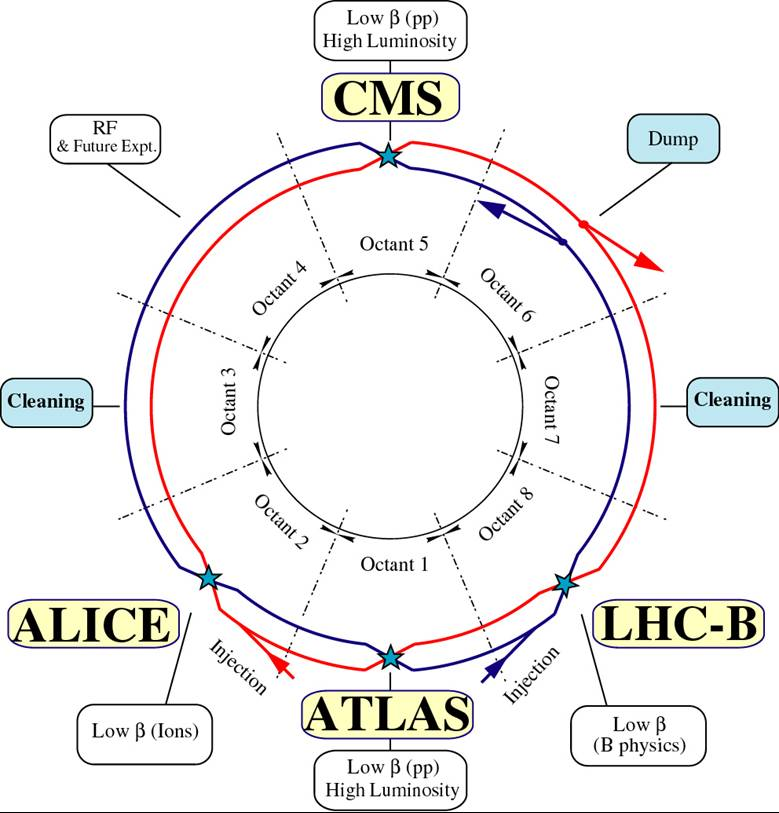
\includegraphics[width=0.7\textwidth]{img/I-2-lhc/lhc.jpg}
		\caption{Schematic representation of the Large Hadron Collider complex under the Franco-Swiss border detailling the location of the four experiment (ALICE, ATLAS, CMS, and LHCb) that analyze the produced collision [CERN].}
		\label{fig:I-2-lhc-schematic}
	\end{figure}

  The construction of the LHC, which concept dates back to 1984, was approved by the CERN Council in December 1994 and started in 1998 with the excavation of the caverns that would hold the experiment sites. In 2003, the first section of the accelerator was assembled inside the tunnel marking the start of the installation phase of the LHC and its detectors which would spawn until 2008. On September 10th 2008, the first beam of protons is circulated inside the LHC only to reveal a major technical issue with the superconducting magnets which will shutdown the machine for nearly a year. In November 2009, reparation works are finished just in time for the LHC to produce its first collisions at 2.36 TeV before its Year End Technical Stop (YETS), a yearly technical stop during which maintainance is performed on the machine. In February 2010, the LHC restarts with a physics program with collisions at 7 TeV that will last until February 2013. At that time, the LHC is stopped for two years during the Long Shutdown (LS) in order to perform upgrades to prepare it to run at 14 TeV. On June 3rd 2015, the LHC restart and sets a new record with an energy in the center of mass reference frame of 13 TeV.

  \section{The Injection Complex}

    The beams that enter the LHC are first created and accelerated by the injection complexe of CERN depicted in Figure \ref{fig:I-2-injection-chain}. Protons are extracted from a gaseous hydrogen source by means of a duoplasmatron, a device that uses a heated filament cathode in conjunction with electric fields to produce electrons that will ionize and break gas. The resulting protons have an energy of 100 keV and are injected in the Linac2 linear accelerator. \\

		\begin{figure}[h!]
			\centering
			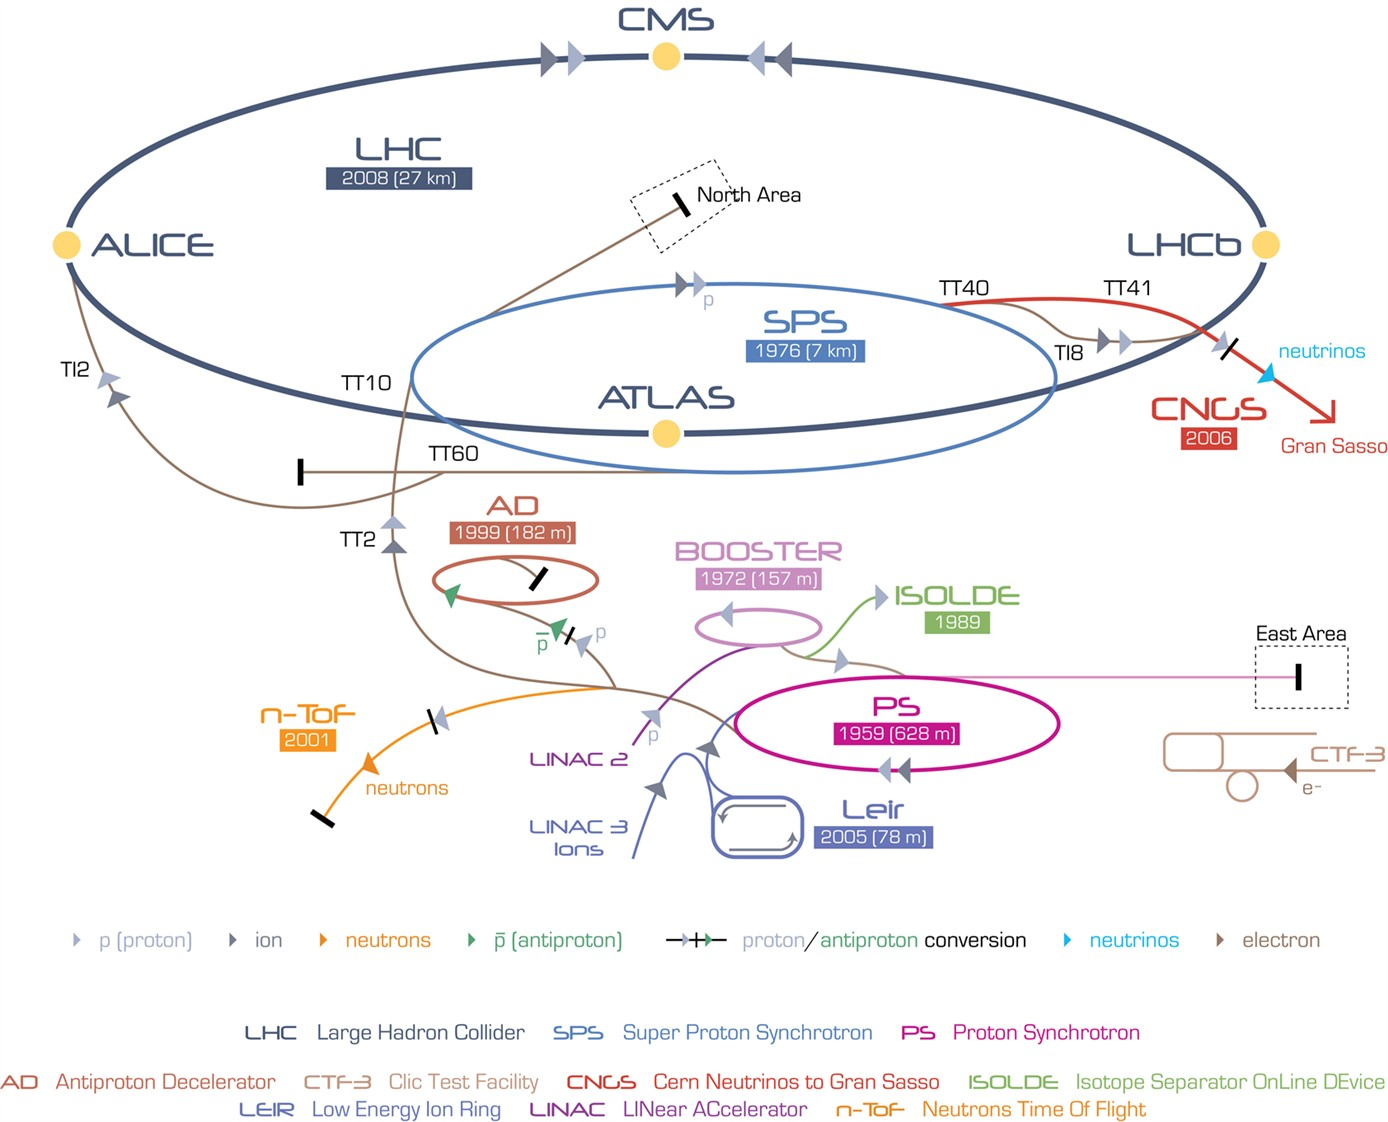
\includegraphics[width = 12cm]{img/I-2-LHC/injectors.png}
			\caption{Schematic representation of the LHC's injection chain composed of multiple smaller accelerators \Cite{TE-EPC-LPC}.}
			\label{fig:I-2-injection-chain}
		\end{figure}

    Linac2 uses radiofrequency cavities that produce an electromagnetic field inside the accelerator in order to transfer energy to the charged particles. The oscillations of the field allow to form bunches of particles by regrouping them on the front of the radio wave. The succession of cavities that form Linac2 boosts the incoming protons to an energy of 50 MeV before they enter the Booster. \\

    Following Linac2, three consecutive circular synchrotrons, namelly the Proton Synchrotron Booster (Booster), the Proton Synchrotron (PS), and the Super Proton Synchrotron (SPS), accelerate the beams to energies of respectivly 1.4 GeV, 25 GeV, and 450 GeV. Each accelerator is composed of electromagnets that bend the trajectory of the beam and boost it further. From the SPS, the beam is injected in the LHC through two transfer tunnels into two rings where they rotate in opposite directions to be further accellerated until they reach the desired energy. The SPS also provides beam to the North Area were various experiments take place and future technologies can be tested during test beam campaignes frequently organised by CERN.

	\section{Preformance Goals}

  	The beams inside the LHC are composed of 2808 bunches, each made of approximatly 110 billion protons, roughtly 30 cm long and separated by 25 ns, time between two consecutive bunch crossing (BX).

    Depending on various parameters, between 20 and 140 proton-proton interactions occur during each bunch crossing (BX).

  	The LHC also delivers a high instantaneous luminosity $ \mathcal{L} $ which is essential to detect rare processes as it yields the apparition's frequency of events in a given interaction process
  	\begin{equation}
  		f_{process} = \mathcal{L} \sigma_{process} \ ,
  	\end{equation}
  	where $ f_{process} $ is the number of expected events per second, and $ \sigma_{process} $ is the interaction cross-section of the process. For a circular collider, the instantaneous luminosity is defined as
  	\begin{equation}
  		\mathcal{L} = \frac{N^2_b n_b f_{rev} \gamma}{4 \pi \epsilon_n \beta^*} F \ ,
  		\label{eq:lhc_and_cms__luminosity}
  	\end{equation}
  	where $ N_b $ is the number of protons or ions per bunch, $ n_b $ is the number of bunches per beam, $ f_{rev} $ is the revolution frequency, $ \gamma $ is the Lorentz factor, $ \epsilon_n $ is the beam emittance, $ \beta^* $ is the beta function at the \emph{Interaction Point} (IP), and $ F $ is a function of the crossing angle between the beams at the IP. The $ \epsilon_n $ and $ F $ parameters are related to the bunches' structure and more specifically to their spatial spreading. These parameters change during the machine's operation as the number of protons per bunch decreases, and the bunches spread out. We can integrate $ \mathcal{L} $ over a long period of time in order to get the integrated luminosity
  	\begin{equation}
  		L = \int \mathcal{L} \ dt \ ,
  	\end{equation}
  	which results in the number of events we can expect for a given interaction process
  	\begin{equation}
  		N_{process} = L \sigma_{process} \ .
  		\label{eq:lhc_and_cms__luminosity_to_N}
  	\end{equation}

	\section{Operations and Schedule}

		The LHC's operation plan \Cite{CMS_Upgrades} is divided in two phases: phase 1 during which the machine will slowly reach its nominal capabilities, and phase 2 where the machine will run at even higher luminosity after undergoing a major upgrade. \\

		Phase 1 extends from 2010 to about 2020 and is divided into three shorter periods separated by two Long Shutdowns. Table \ref{tab:lhc_and_cms__lhc_performances} shows the energy and luminosity at which the LHC will be running after both maintenances (LS1 and LS2). While the machine is shut down, physicists will have access to the detectors and will be able to perform repairs and upgrades. \\

		\begin{table}[h!]
			\centering
			\begin{tabular}{l|c|c}
				Period & Energy & Luminosity \\ \hline
				2010-2012 & 7-8 TeV & 0.5 10$ ^{34} $ cm$ ^{-2} $ s$ ^{-1} $ \\
				Long Shutdown 1 (LS1) & - & - \\
				2015-2017 & 13-14 TeV & 10$ ^{34} $ cm$ ^{-2} $ s$ ^{-1} $ \\
				Long Shutdown 2 (LS2) & - & - \\
				2019-2021 & 14 TeV & 2 10$ ^{34} $ cm$ ^{-2} $ s$ ^{-1} $
			\end{tabular}
			\caption{Energy and luminosity of the LHC during the different periods of phase 1 \Cite{LHC_Machine}.}
			\label{tab:lhc_and_cms__lhc_performances}
		\end{table}

		After LS1, the energy will be increased by using the magnets at full capability, and the luminosity will be multiplied by a factor of two by bringing down the time between two collisions to 25 ns instead of 50 ns. The luminosity will further be increased after LS2 when the machine enters the \emph{High Luminosity LHC} (HL-LHC) era. As reviewed in Equation \ref{eq:lhc_and_cms__luminosity}, various parameters can be tuned in order to achieve that goal. The main possibilities are to \Cite{LHC_LS1, LHC_Upgrade_Scenarios}
		\begin{enumerate}
			\item increase the number of bunches $ \sim n_b $;
			\item increase the number of protons per bunch by making them longer $ \sim N_b $;
			\item increase the collisions' frequency $ \sim f_{rev} $;
			\item decrease the bunches' spread by improving the efficiency of the focusing magnets $ \sim \epsilon_n $;
			\item decrease the collisions' angle by adding magnets near the IPs $ \sim F $. \\
		\end{enumerate}

		Phase 2 involves a major upgrade of the LHC and of the injection chain which would occur during LS3 after 2021. The objective is to increase the luminosity by a factor of 10 to reach 10$ ^{35} $ cm$ ^{-2} $ s$ ^{-1} $.
